\documentclass[11pt, letterpaper]{article}
\usepackage[utf8]{inputenc}
\usepackage{geometry}
\usepackage{fancyhdr}
\usepackage{amsmath, amssymb}
\usepackage{xcolor}
\usepackage{listings}
\usepackage{enumitem}
\usepackage{hyperref}
\usepackage{booktabs}
\usepackage{graphicx}

\setlength{\parindent}{0pt}
\setlist{itemsep=0.5em}
\setlength{\parskip}{0.5em}

\geometry{margin=1in}
\pagestyle{fancy}
\fancyhf{}
\lhead{\textbf{Solutions}}
\rhead{\textbf{Data Analysis and Regression, Homework 5}}
\cfoot{\thepage}

\definecolor{codegreen}{rgb}{0,0.6,0}
\definecolor{codegray}{rgb}{0.5,0.5,0.5}
\definecolor{codepurple}{rgb}{0.58,0,0.82}
\definecolor{backcolour}{rgb}{0.95,0.95,0.92}

\lstdefinestyle{mystyle}{
    backgroundcolor=\color{backcolour},   
    commentstyle=\color{codegreen},
    keywordstyle=\color{magenta},
    numberstyle=\tiny\color{codegray},
    stringstyle=\color{codepurple},
    basicstyle=\ttfamily\footnotesize,
    breakatwhitespace=false,         
    breaklines=true,                 
    captionpos=b,                    
    keepspaces=true,                 
    numbers=left,                    
    numbersep=5pt,                  
    showspaces=false,                
    showstringspaces=false,
    showtabs=false,                  
    tabsize=2
}
\lstset{style=mystyle}

\newcommand{\problem}[1]{\section*{Problem #1}}
\newcommand{\subproblem}[1]{\subsection*{Problem #1}}
\newcommand{\answer}{\textbf{\textit{\textcolor{red}{Answer:}}}}
\begin{document}

\section*{Instructions}
\begin{itemize}
    \item Homework 5 was due Wednesday, August 26th at 18:00 Chicago Time.
    \item All numbers and figures come from \texttt{homework\_5\_solution.ipynb}, run from top to bottom.
\end{itemize}
\hrule
\vspace{0.5cm}

\pagebreak

\problem{1: PCA from Scratch}

In this problem, you will implement Principal Component Analysis (PCA) ``by hand'' (using basic linear algebra functions) and compare it to the standard implementation.

Generate a dataset with $n=500$ observations and 3 highly correlated features.
$$ \mu = [0, 0, 0] $$
$$ \Sigma = \begin{pmatrix} 1 & 0.9 & 0.7 \\ 0.9 & 1 & 0.8 \\ 0.7 & 0.8 & 1 \end{pmatrix} $$

    \begin{lstlisting}[language=Python]
import numpy as np
np.random.seed(42)
mean = [0, 0, 0]
cov = [[1, 0.9, 0.7], [0.9, 1, 0.8], [0.7, 0.8, 1]]
X = np.random.multivariate_normal(mean, cov, 500)\end{lstlisting}

\subproblem{1.1: Eigendecomposition}
\begin{itemize}
    \item Calculate the covariance matrix of the data $X$ manually (recall $\text{Cov}(X) = \frac{1}{n-1}X^T X$ if $X$ is centered).
    \item Find the eigenvalues and eigenvectors of this covariance matrix using \texttt{np.linalg.eig}.
    \item Report the eigenvalues and eigenvectors.
\end{itemize}

\answer

The covariance matrix is symmetric, so use \texttt{np.linalg.eigh}: it returns real eigenvalues in
ascending order. \texttt{np.linalg.eig} is the general routine, and here it returns complex dtype in
no particular order.

\begin{lstlisting}[language=Python]
X_demeaned = X - X.mean(axis=0)
covX = 1 / 499 * X_demeaned.T @ X_demeaned

eigenvalues, eigenvectors = np.linalg.eigh(covX)
order = np.argsort(eigenvalues)[::-1]
eigenvalues, eigenvectors = eigenvalues[order], eigenvectors[:, order]
\end{lstlisting}

Sorted largest first:
\[
\lambda = (2.290778,\; 0.313006,\; 0.087826),
\qquad
Q = \begin{bmatrix}
-0.585990 & -0.571257 & -0.574701 \\
-0.604994 & -0.163388 &  0.779286 \\
-0.539071 &  0.804345 & -0.249863
\end{bmatrix}
\]
where the columns of $Q$ are the eigenvectors in the same order. The three features are strongly
correlated, so PC1 alone carries $85.1\%$ of the variance, against $11.6\%$ and $3.3\%$ for the
other two.


\subproblem{1.2: Projection}
\begin{itemize}
    \item Project the data $X$ onto the principal components (the eigenvectors). 
    \item Plot the original data (pick any 2 dimensions) and the projected data (PC1 vs PC2).
\end{itemize}

\answer

\begin{center}
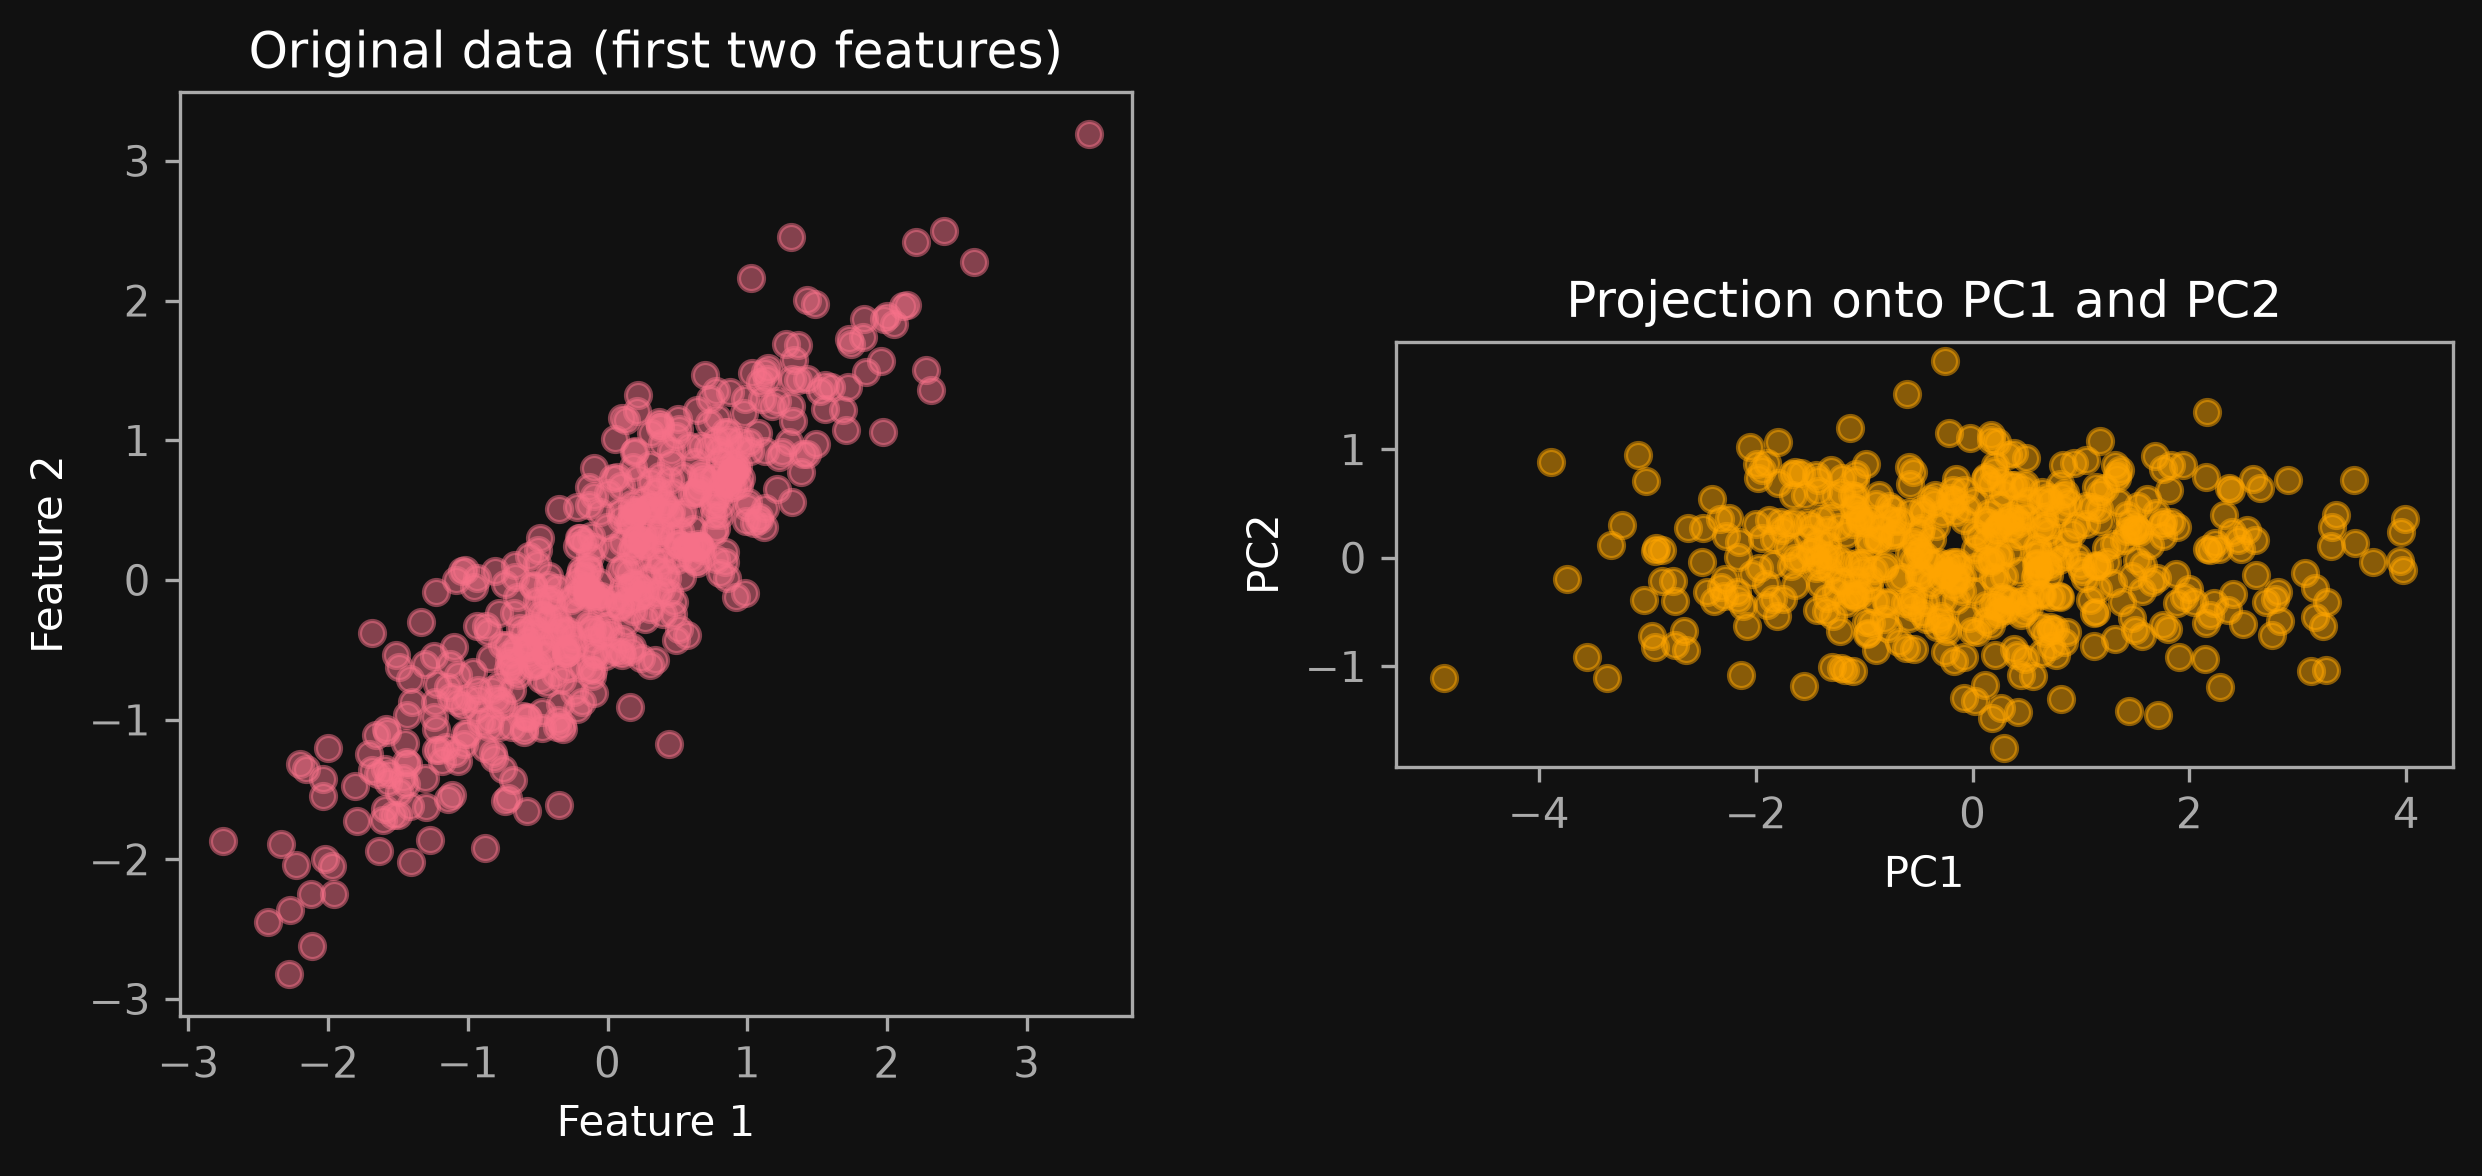
\includegraphics[width=0.95\textwidth]{./figures/problem1_pca_projection.png}
\end{center}

Both panels are drawn on equal axes. The raw features lie on a tilted cigar, because they are
correlated. Rotating onto the eigenvectors removes the tilt: PC1 and PC2 are uncorrelated by
construction, and almost all of the spread has been moved onto PC1.


\subproblem{1.3: Verification}
\begin{itemize}
    \item Use \texttt{sklearn.decomposition.PCA} to perform PCA on the same data.
    \item Compare the components (eigenvectors) and explained variance (eigenvalues) from \texttt{sklearn} with your manual calculation. Are they the same?
\end{itemize}

\answer

Yes. The eigenvalues agree with \texttt{pca.explained\_variance\_} to
$4.4 \times 10^{-16}$, and the eigenvectors agree with \texttt{pca.components\_} up to a sign flip
on PC1.

The sign is arbitrary: if $v$ is a unit eigenvector then so is $-v$, and nothing in the
decomposition prefers one. \texttt{sklearn} pins it down by a convention on the loadings;
\texttt{eigh} does not.


\problem{2: The Pitfalls of Principal Component Regression (PCR)}

A common misconception is that the principal components with the largest variance are always the most useful features for prediction. This problem illustrates a scenario where this is \textbf{not} true.

Generate the following dataset:

    \begin{lstlisting}[language=Python]
import numpy as np
import pandas as pd
import statsmodels.api as sm
from sklearn.decomposition import PCA

np.random.seed(42)
n = 500

X_high_var = np.random.normal(0, 10, (n, 7))
X_low_var = np.random.normal(0, 1, (n, 3))
X = np.hstack([X_high_var, X_low_var])

true_beta = np.array([0]*7 + [2, -2, 2])
y = X @ true_beta + np.random.normal(0, 0.5, n)\end{lstlisting}

\subproblem{2.1: PCA Analysis}
Run PCA on the raw input matrix $X$. You must center the data first ($\tilde{X} = X - \bar{X}$). 
\begin{itemize}
    \item Report the explained variance ratio for all 10 components.
    \item Which components capture the majority of the variance?
\end{itemize}

\answer

\begin{center}
\begin{tabular}{lr}
\toprule
 & explained variance ratio \\
\midrule
PC1 & 0.16773 \\
PC2 & 0.16159 \\
PC3 & 0.15787 \\
PC4 & 0.14255 \\
PC5 & 0.12969 \\
PC6 & 0.12647 \\
PC7 & 0.10983 \\
PC8 & 0.00149 \\
PC9 & 0.00142 \\
PC10 & 0.00136 \\
\bottomrule
\end{tabular}
\end{center}

PC1 to PC7 hold $99.57\%$ of the variance, PC8 to PC10 the remaining $0.43\%$. The split is
mechanical: the first seven columns of $X$ were drawn with $\sigma = 10$ and the last three with
$\sigma = 1$, a variance ratio of $100$ to $1$.


\subproblem{2.2: PCR - Regressing on High Variance Components}
Fit an OLS model using \textbf{only} the first 7 principal components to predict $y$.
\begin{itemize}
    \item Report the $R^2$ of this model.
    \item Does capturing the majority of the variance ensure good predictive power?
\end{itemize}

\answer

$R^2 = \mathbf{0.0064}$.

No. Those seven components hold $99.57\%$ of the variance in $X$ and explain $0.6\%$ of $y$. PCA
never looks at $y$, so ranking components by variance ranks them by how much they move, not by how
much they matter.


\subproblem{2.3: PCR - Regressing on Low Variance Components}
Fit an OLS model using \textbf{only} the last 3 principal components (PC8, PC9, PC10) to predict $y$.
\begin{itemize}
    \item Report the $R^2$ of this model.
\end{itemize}

\answer

$R^2 = \mathbf{0.9750}$, from the three components that carry $0.43\%$ of the variance.


\subproblem{2.4: Conclusion}
Based on your results, explain why simply selecting the top $k$ principal components for a regression model might be dangerous.

\answer

Because variance in $X$ and predictive power for $y$ are unrelated quantities, and here they are
exactly reversed: the top seven components give $R^2 = 0.0064$ and the bottom three give
$R^2 = 0.9750$. Truncating at the top $k$ would have thrown away the entire signal while keeping
all of the noise.

Variance also depends on units. Rescaling one column in meters rather than kilometers changes its
variance by $10^6$ and reorders the components, without changing the regression at all.

If the goal is prediction, select on something that sees $y$: cross-validated Lasso, partial least
squares, or cross-validating over which components to keep rather than assuming the top ones.


\problem{3: Bagging from Scratch}

In class, we discussed how Bagging (Bootstrap Aggregating) reduces variance by averaging predictions from multiple models trained on bootstrapped samples. You will implement this manually.

Generate a synthetic ``checkerboard'' dataset:
    \begin{lstlisting}[language=Python]
import pandas as pd
np.random.seed(42)
n_points = 500
grid_size = 4
limit = 10
step = (limit * 2) / grid_size

all_points = []
all_labels = []

for i in range(grid_size):
    for j in range(grid_size):
        label = (i + j) % 2
        x_min, x_max = -limit + i * step, -limit + (i + 1) * step
        y_min, y_max = -limit + j * step, -limit + (j + 1) * step
        points_x = np.random.uniform(x_min, x_max, int(n_points/16))
        points_y = np.random.uniform(y_min, y_max, int(n_points/16))
        all_points.append(np.vstack((points_x, points_y)).T)
        all_labels.extend([label] * int(n_points/16))

X = np.vstack(all_points)
y = np.array(all_labels)\end{lstlisting}

\subproblem{3.1: Single Decision Tree}
Fit a single \texttt{DecisionTreeClassifier} (from \texttt{sklearn}) with \texttt{max\_depth=None} (or a high number like 10) to the data.
\begin{itemize}
    \item Visualize the decision boundary (you can use the meshgrid method shown in class).
    \item Does the decision boundary look smooth? Does it look like it's overfitting?
\end{itemize}

\answer

\begin{center}
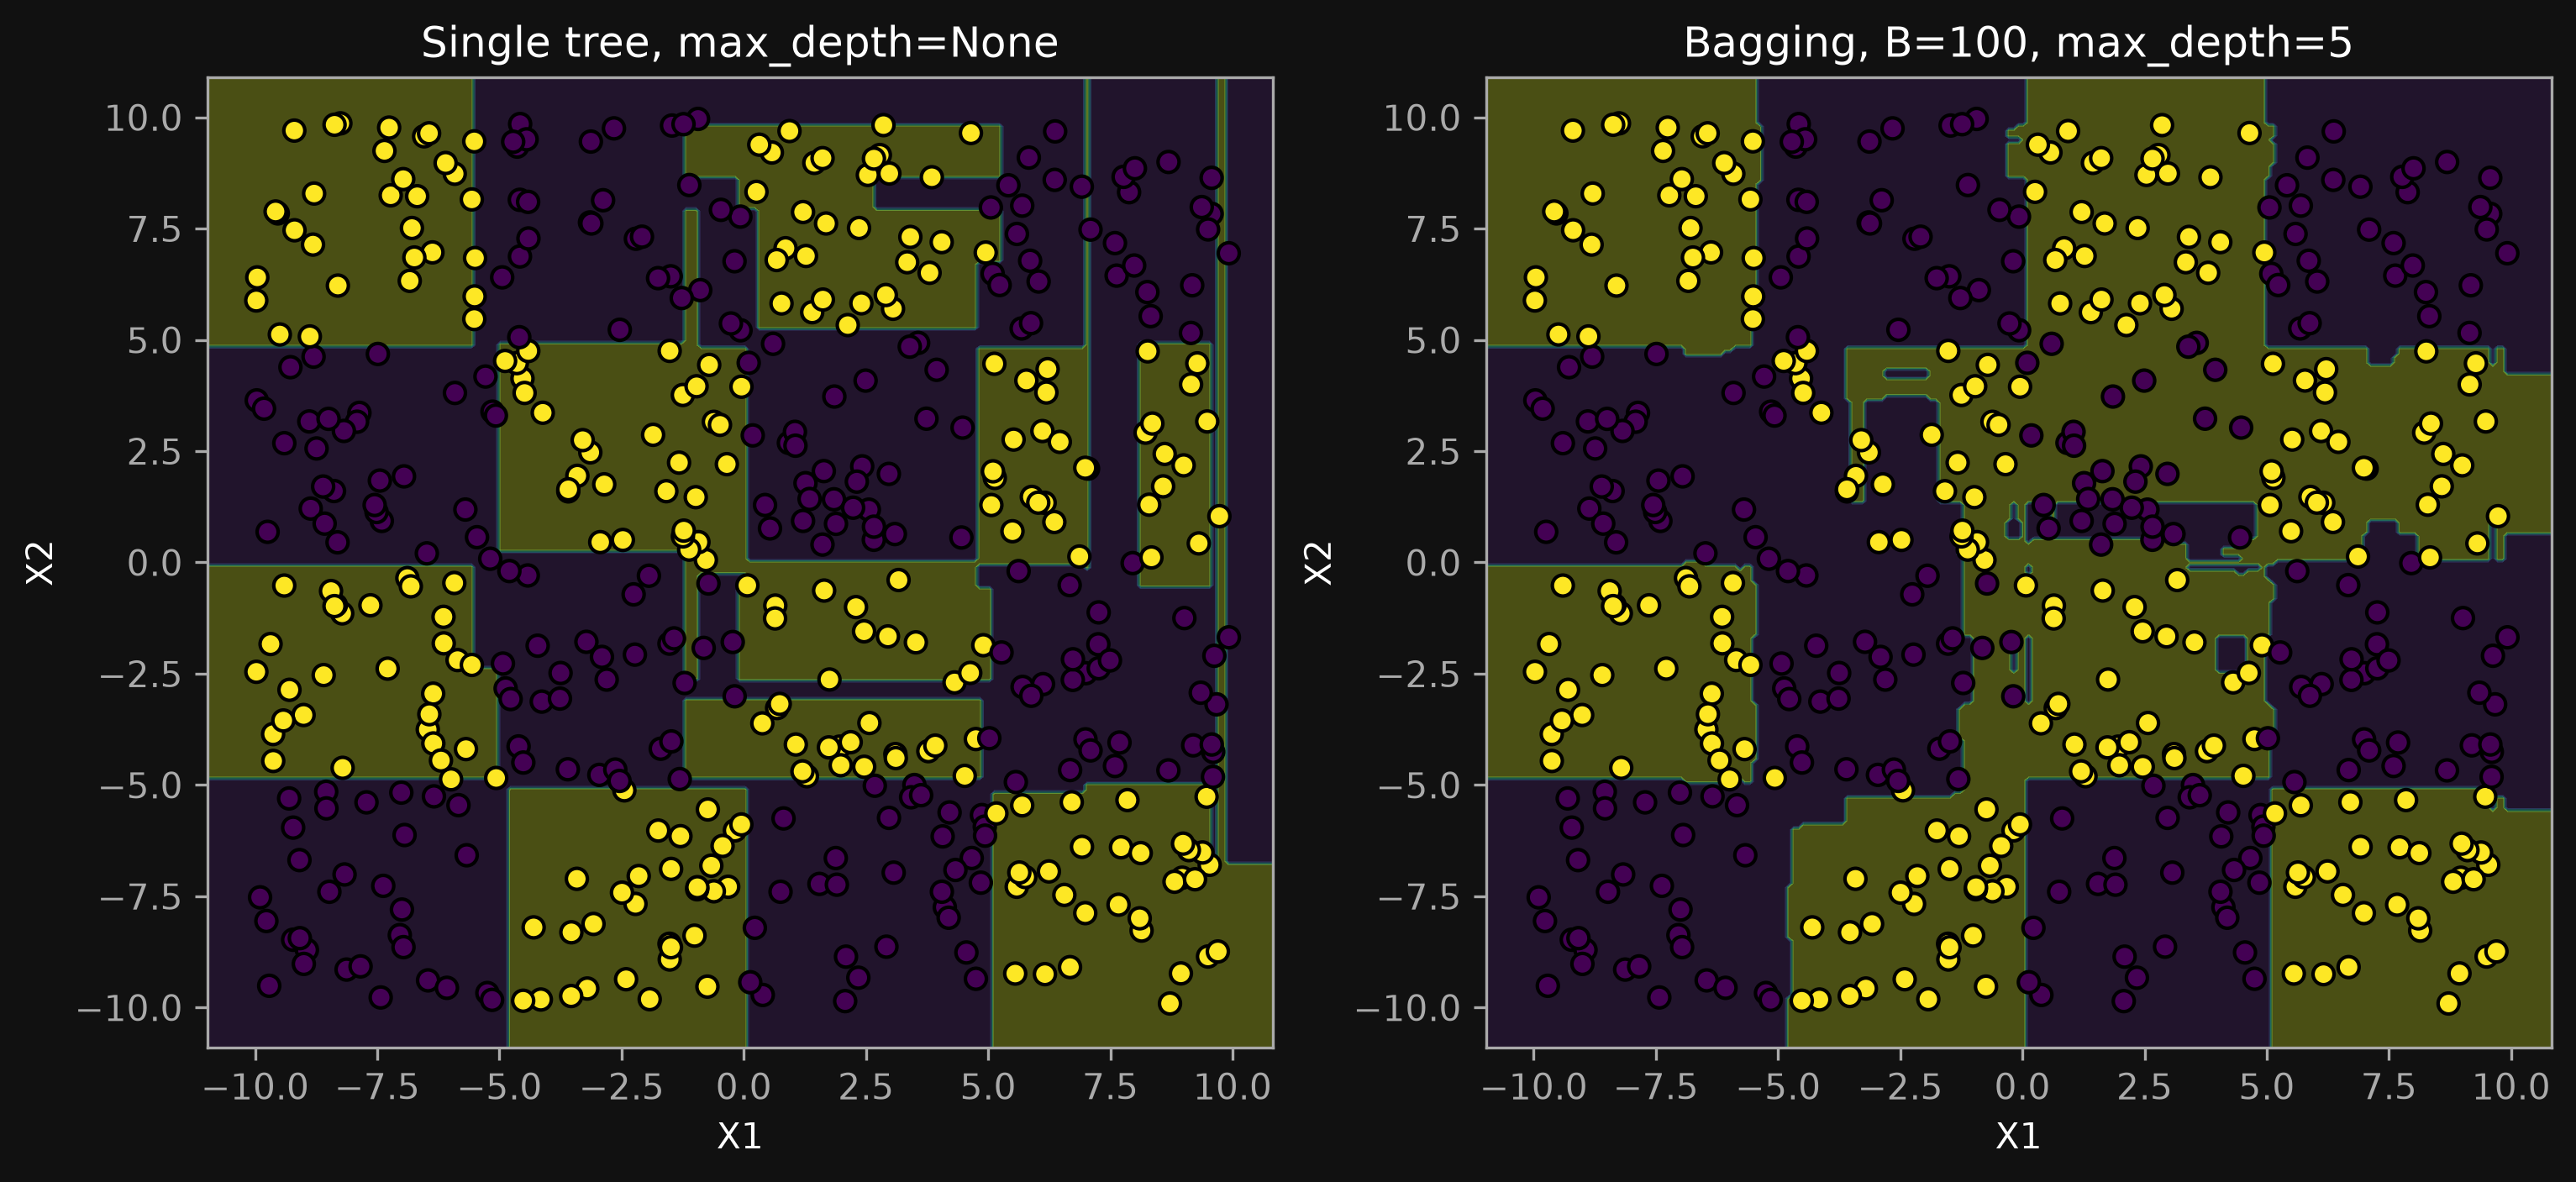
\includegraphics[width=0.95\textwidth]{./figures/problem3_bagging_comparison.png}
\end{center}

Not smooth, and yes it is overfitting. The boundary is a staircase of axis-aligned rectangles, and
several are thin slivers wrapped around one or two points, well inside a square where every point
carries the same label. Training accuracy is $1.0000$: with \texttt{max\_depth=None} the tree splits
until every leaf is pure, so it reproduces the noise as well as the checkerboard.


\subproblem{3.2: Manual Bagging Implementation}
Implement Bagging manually (do \textbf{not} use \texttt{BaggingClassifier}).
\begin{itemize}
    \item Create a loop that runs $B=100$ times.
    \item Inside the loop:
    \begin{enumerate}
        \item Create a bootstrap sample of the dataset (sample $N$ rows with replacement).
        \item Fit a new \texttt{DecisionTreeClassifier} (max\_depth=5) on this bootstrap sample.
        \item Store the trained tree in a list.
    \end{enumerate}
    \item To predict for a new point (or the meshgrid for plotting), get predictions from all 100 trees and take the majority vote (average).
\end{itemize}

Visualize the decision boundary of your manual Bagging ensemble.

\answer

The ensemble boundary is the right-hand panel of the figure above.

\begin{lstlisting}[language=Python]
class BaggingDTC:
    def __init__(self, B=100, max_depth=5, seed=0):
        self.B = B
        self.max_depth = max_depth
        self.rng = np.random.RandomState(seed)
        self.trees = []

    def fit(self, X, y):
        n_samples = X.shape[0]
        for _ in range(self.B):
            idx = self.rng.choice(n_samples, size=n_samples, replace=True)
            tree = DecisionTreeClassifier(max_depth=self.max_depth, random_state=42)
            self.trees.append(tree.fit(X[idx], y[idx]))
        return self

    def predict(self, X):
        votes = np.array([tree.predict(X) for tree in self.trees])
        return (votes.mean(axis=0) >= 0.5).astype(int)
\end{lstlisting}


\subproblem{3.3: Comparison and Interpretation}
Compare the decision boundary of your Bagging ensemble to the single decision tree in 3.1. Is it smoother? Relate what you see to variance reduction.

\answer

Yes. The slivers are gone and the boundary sits close to the true grid lines at $\pm 5$ and $0$.

Each bootstrap sample omits about $37\%$ of the data, so each tree puts its spurious splits in a
different place. Those splits are variance, not signal, and they do not survive a vote across 100
trees, while the real boundaries appear in nearly every tree and do. Averaging $B$ predictors
reduces the variance of the average without changing its expectation, which is the whole mechanism.

Training accuracy falls from $1.0000$ to $0.9194$. That is the trade: the ensemble gives up fitting
the training labels exactly in exchange for a boundary that reflects the generating process.


\problem{4: Gradient Boosting from Scratch}

We often use OLS because it is simple and interpretable. However, it can suffer from high bias if the true relationship is non-linear. In this problem, you will implement Gradient Boosting manually to correct the bias of an OLS model.

Generate the following non-linear dataset:
    \begin{lstlisting}[language=Python]
import numpy as np
import matplotlib.pyplot as plt
from sklearn.linear_model import LinearRegression
from sklearn.tree import DecisionTreeRegressor

np.random.seed(42)
X = np.linspace(0, 10, 100).reshape(-1, 1)
# y is exponential, which OLS struggles with
y = np.exp(X.ravel() / 3) + np.random.normal(0, 0.5, 100)\end{lstlisting}

\subproblem{4.1: The Base Model (OLS)}
\begin{itemize}
    \item Fit a standard Linear Regression (OLS) model to $X$ and $y$.
    \item Calculate and report the Mean Squared Error (MSE).
    \item Plot the data and the OLS prediction line. Observe how the straight line fails to capture the curve (high bias).
\end{itemize}

\answer

$\text{MSE} = \mathbf{8.2298}$.

\begin{center}
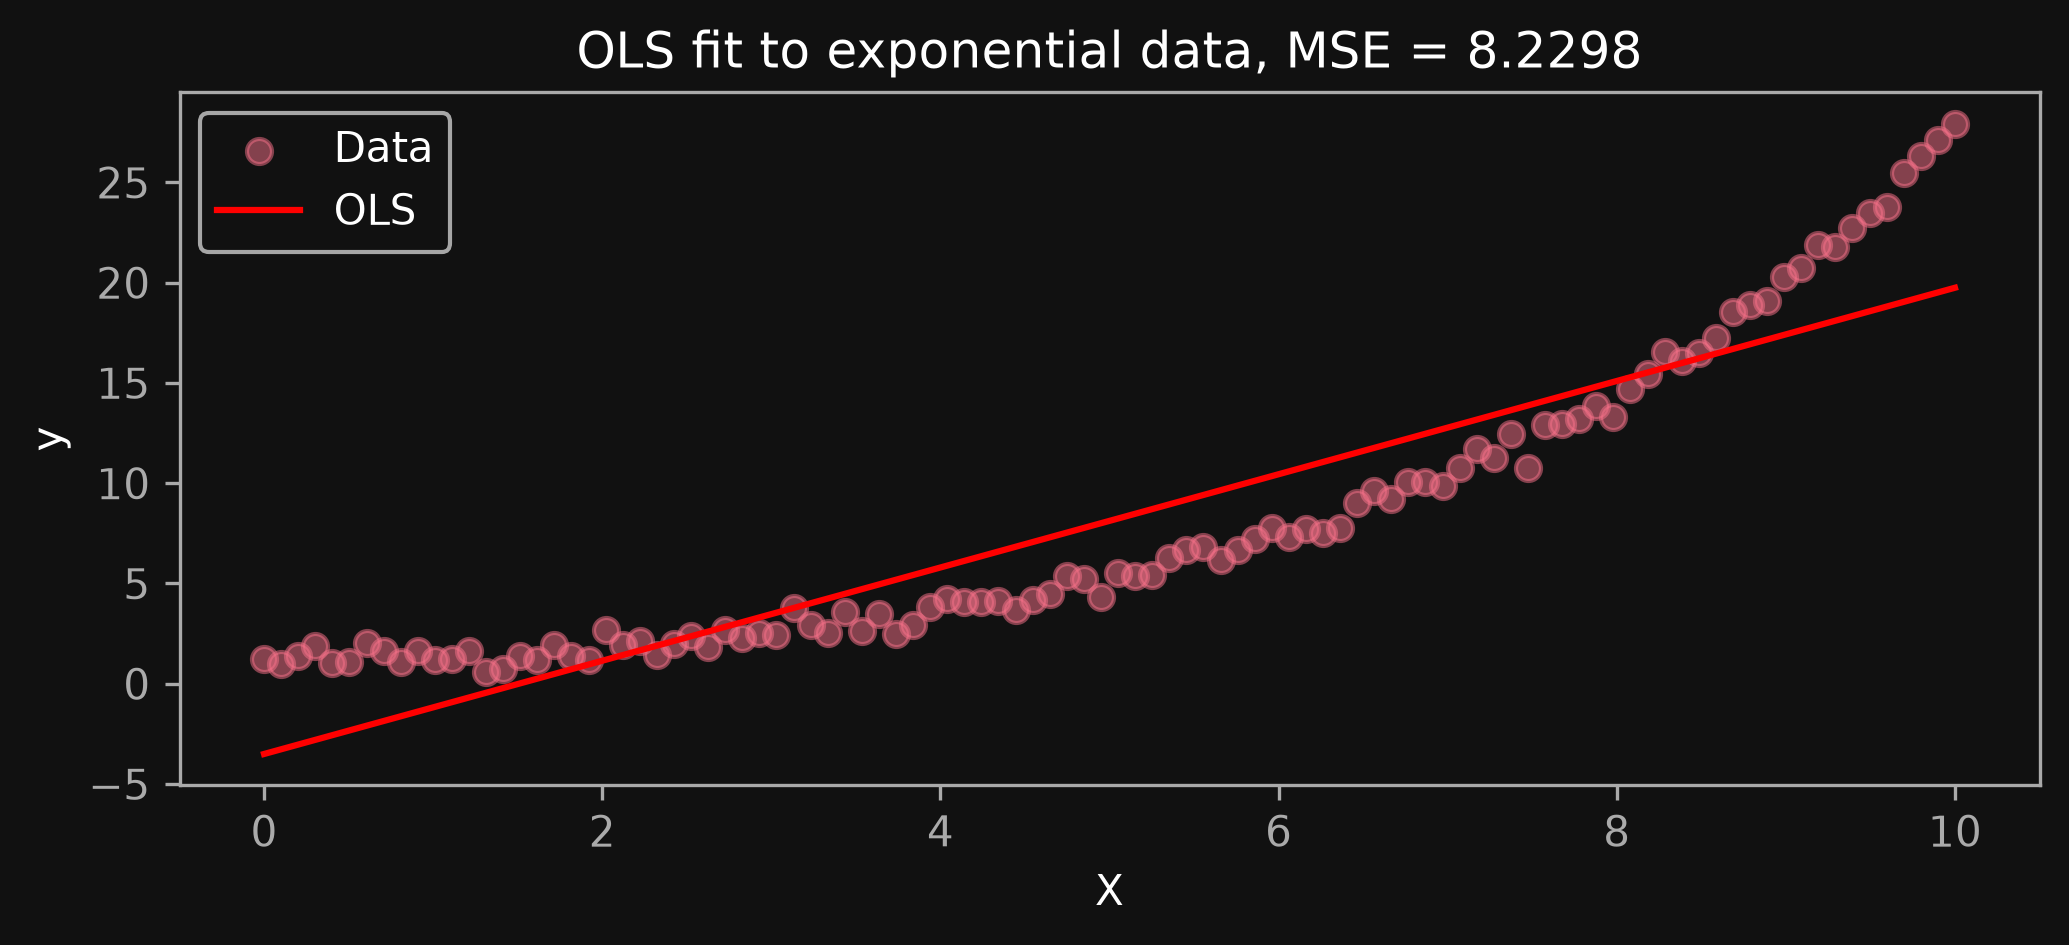
\includegraphics[width=0.95\textwidth]{./figures/problem4_ols_fit.png}
\end{center}

The line cuts through the curve: it sits below the data at both ends and above it in the middle, so
the residuals are a smooth function of $X$ rather than noise. That is what high bias looks like --
the error is in the shape of the model, and no amount of extra data would remove it.


\subproblem{4.2: Boosting with Residuals}
Now, we will boost this model by iteratively fitting the residuals with weak learners (shallow trees).

Implement the following algorithm:
\begin{enumerate}
    \item Initialize predictions with the OLS model: $F_0(x) = \hat{y}_{OLS}$.
    \item Set learning rate $\eta = 0.1$.
    \item Loop 50 times ($m=1$ to $50$):
    \begin{itemize}
        \item Calculate residuals: $r_m = y - F_{m-1}(x)$.
        \item Fit a \texttt{DecisionTreeRegressor} with \texttt{max\_depth=1} to the data $(X, r_m)$. This is your weak learner $h_m(x)$.
        \item Update predictions: $F_m(x) = F_{m-1}(x) + \eta \cdot h_m(x)$.
    \end{itemize}
\end{enumerate}

\answer

\begin{lstlisting}[language=Python]
pred = ols.fittedvalues.copy()
eta = 0.1
for _ in range(50):
    resid_m = y - pred
    tree = DecisionTreeRegressor(max_depth=1, random_state=0).fit(X, resid_m)
    pred = pred + eta * tree.predict(X)
\end{lstlisting}


\subproblem{4.3: Results}
\begin{itemize}
    \item Plot the final boosted prediction $F_{50}(x)$ against the original data.
    \item Calculate the final MSE. Compare it to the OLS MSE.
    \item Explain intuitively what the boosting process did to the original linear line.
\end{itemize}

\answer

$\text{MSE}$ falls from $8.2298$ to $\mathbf{0.7754}$, a factor of $10.6$.

\begin{center}
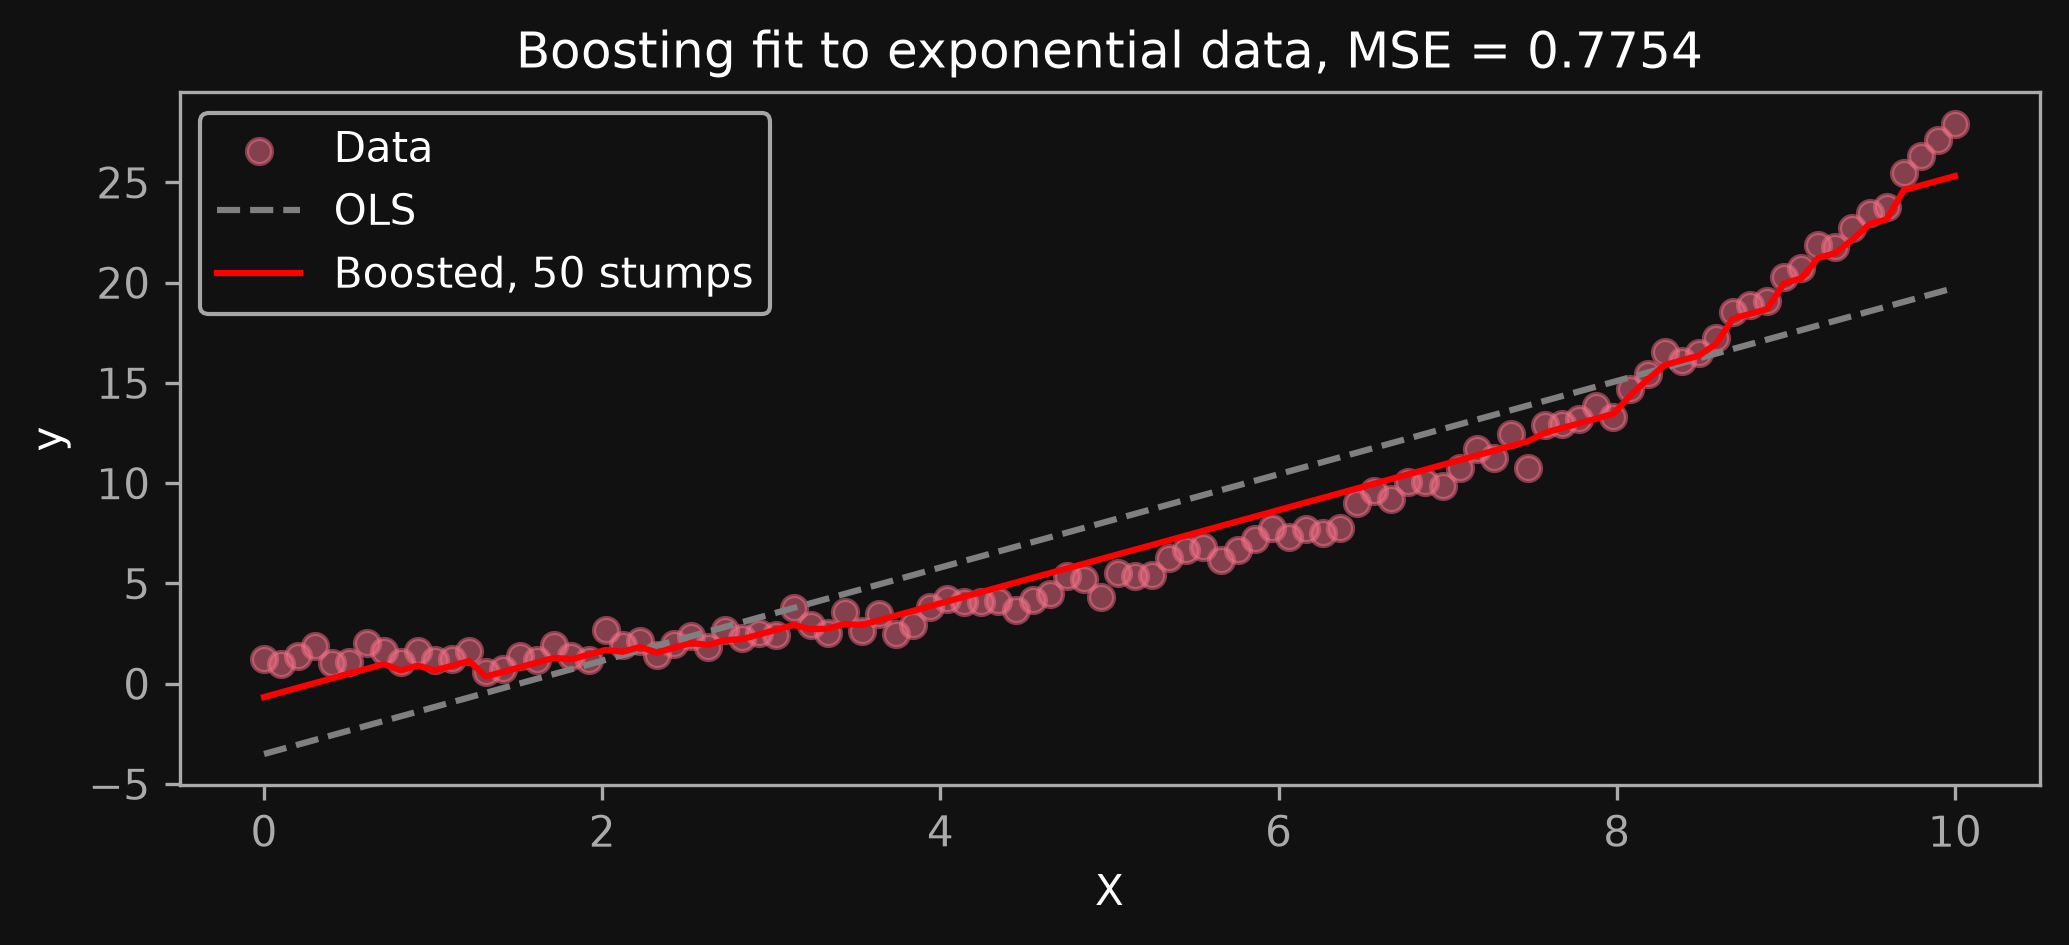
\includegraphics[width=0.95\textwidth]{./figures/problem4_boosting_fit.png}
\end{center}

Each stump is one split on $X$, so it adds one small step to the prediction, placed wherever the
current residuals are most lopsided. Fifty of those steps at $\eta = 0.1$ accumulate into a
staircase that bends the straight line into the exponential.

The correction is applied where the line was wrong: the steps pile up at the right-hand end, where
OLS underfits worst. Nothing here changed the model class -- the base learner is still a line, and
the trees are fitted to what the line got wrong.


\problem{5: Boosting vs. Random Forest}

Using the same dataset as Problem 3 (the checkerboard), we will compare Random Forest (which uses Bagging + feature splitting) and AdaBoost (which reduces bias).

\subproblem{5.1: Model Comparison}
\begin{itemize}
    \item Fit a \texttt{RandomForestClassifier} with 100 estimators.
    \item Fit an \texttt{AdaBoostClassifier} with 50 estimators (base estimator can be a Tree with depth 3).
    \item Report the accuracy of both models on the dataset (since we didn't do a train/test split, reporting training accuracy is fine for this illustrative comparison).
\end{itemize}

\answer

\begin{center}
\begin{tabular}{lrr}
\toprule
 & in-sample & held out (70/30) \\
\midrule
Random Forest & 1.0000 & 0.8792 \\
AdaBoost & 1.0000 & 0.8389 \\
\bottomrule
\end{tabular}
\end{center}

Both models reach $1.0000$ in sample, so as the question warns, that column cannot separate them:
100 unpruned trees and 50 depth-3 trees are both large enough to memorize 496 points.

The held-out column is added because of that. On a $70/30$ split ($347$ train, $149$ test) the
random forest reaches $0.8792$ against $0.8389$ for AdaBoost.


\subproblem{5.2: Conceptual Question}
Explain in 2-3 sentences:
\begin{itemize}
    \item Why does Random Forest help reduce \textit{variance}?
    \item Why does Boosting help reduce \textit{bias}?
\end{itemize}

\answer

\textbf{Random Forest reduces variance.} Each tree is fitted to a bootstrap sample and each split
sees a random subset of features, so the trees make different mistakes. Averaging $B$ predictors
with correlation $\rho$ leaves variance $\rho\sigma^2 + (1-\rho)\sigma^2/B$: bagging supplies the
$1/B$ term and the random feature subset lowers $\rho$, which is what the extra randomization buys
over plain bagging. It does not touch bias -- the average of $B$ trees has the bias of one tree.

\textbf{Boosting reduces bias.} Each round fits the residuals of what is already there, so the
ensemble keeps adding structure the current model is missing. Fifty depth-3 stumps can represent
shapes no single depth-3 tree can. The cost is the mirror image: errors accumulate rather than
average out, so boosting will fit noise if run too long, and it needs a learning rate or an early
stop to hold it back.


\problem{6: Clustering from Scratch (DBSCAN Flavor)}

Standard K-Means clustering assumes that clusters are spherical and roughly the same size. 
DBSCAN is an alternative that finds clusters of arbitrary shape. You will implement a simplified version of this.

Generate the ``Moons" dataset:
    \begin{lstlisting}[language=Python]
from sklearn.datasets import make_moons
import numpy as np
import matplotlib.pyplot as plt

np.random.seed(42)
X, _ = make_moons(n_samples=300, noise=0.05)\end{lstlisting}

\subproblem{6.1: The Algorithm}
It may be helpful to cache the pairwise distances between points to speed up the algorithm,
you can do this using \texttt{scipy.spatial.distance.cdist} or numpy operations.

Implement the following simplified DBSCAN logic:
\begin{itemize}
    \item Set $\epsilon = 0.2$ and $\text{MinPts} = 5$.
    \item Initialize all points as unvisited.
    \item Initialize \texttt{cluster\_id = 0}.
    \item Loop through each point $P$ in $X$:
    \begin{itemize}
        \item If $P$ is visited, continue.
        \item Mark $P$ as visited.
        \item Find all neighbors of $P$ within distance $\epsilon$.
        \item If number of neighbors $< \text{MinPts}$, mark $P$ as Noise (Cluster \texttt{-1}).
        \item If number of neighbors $\ge \text{MinPts}$:
        \begin{itemize}
            \item Increment \texttt{cluster\_id}.
            \item Assign $P$ to \texttt{cluster\_id}.
            \item Expand the cluster (Breadth-First Search): Add all neighbors to a queue. For each point $Q$ in the queue:
            \begin{itemize}
                \item If $Q$ is unvisited, mark it visited.
                \item If $Q$ has enough neighbors ($\ge \text{MinPts}$), add those neighbors to the queue.
                \item If $Q$ is not yet assigned to a cluster, assign it to \texttt{cluster\_id}.
            \end{itemize}
        \end{itemize}
    \end{itemize}
\end{itemize}

\answer

\begin{lstlisting}[language=Python]
def cdist(a, b):
    return np.sqrt(((a[:, np.newaxis, :] - b[np.newaxis, :, :]) ** 2).sum(axis=2))

eps = 0.2
min_pts = 5
labels = np.full(X_moons.shape[0], -2)  # -2: unvisited, -1: noise
cluster_id = -1
dists = cdist(X_moons, X_moons)

for i in range(len(X_moons)):
    if labels[i] != -2:
        continue
    neighbors = np.where(dists[i] < eps)[0]
    if len(neighbors) < min_pts:
        labels[i] = -1  # noise, but may still be claimed as a border point below
    else:
        cluster_id += 1
        labels[i] = cluster_id
        queue = list(neighbors)
        while queue:
            q = queue.pop(0)
            if labels[q] >= 0:
                continue  # already in a cluster
            labels[q] = cluster_id  # unvisited, or previously marked noise
            q_neighbors = np.where(dists[q] < eps)[0]
            if len(q_neighbors) >= min_pts:
                queue.extend(q_neighbors)
\end{lstlisting}

The test inside the queue is \texttt{labels[q] >= 0}, not \texttt{labels[q] != -2}. A point marked
noise earlier can still be a border point of a cluster found later, and that is the behavior
\texttt{sklearn} implements. Caching the full distance matrix once turns the neighbor lookup into
an $O(1)$ row read.


\subproblem{6.2: Visualization}
\begin{itemize}
    \item Plot the points $X$, colored by their assigned cluster labels.
    \item Verify using \texttt{sklearn.cluster.DBSCAN} with the same parameters. Do the plots look the same?
\end{itemize}

\answer

Identical. Both give two clusters of exactly $150$ points and no noise, and
\texttt{np.array\_equal(labels, labels\_sklearn)} is \texttt{True} -- the cluster ids happen to line
up too, since both algorithms number clusters in order of first visit.

\begin{center}
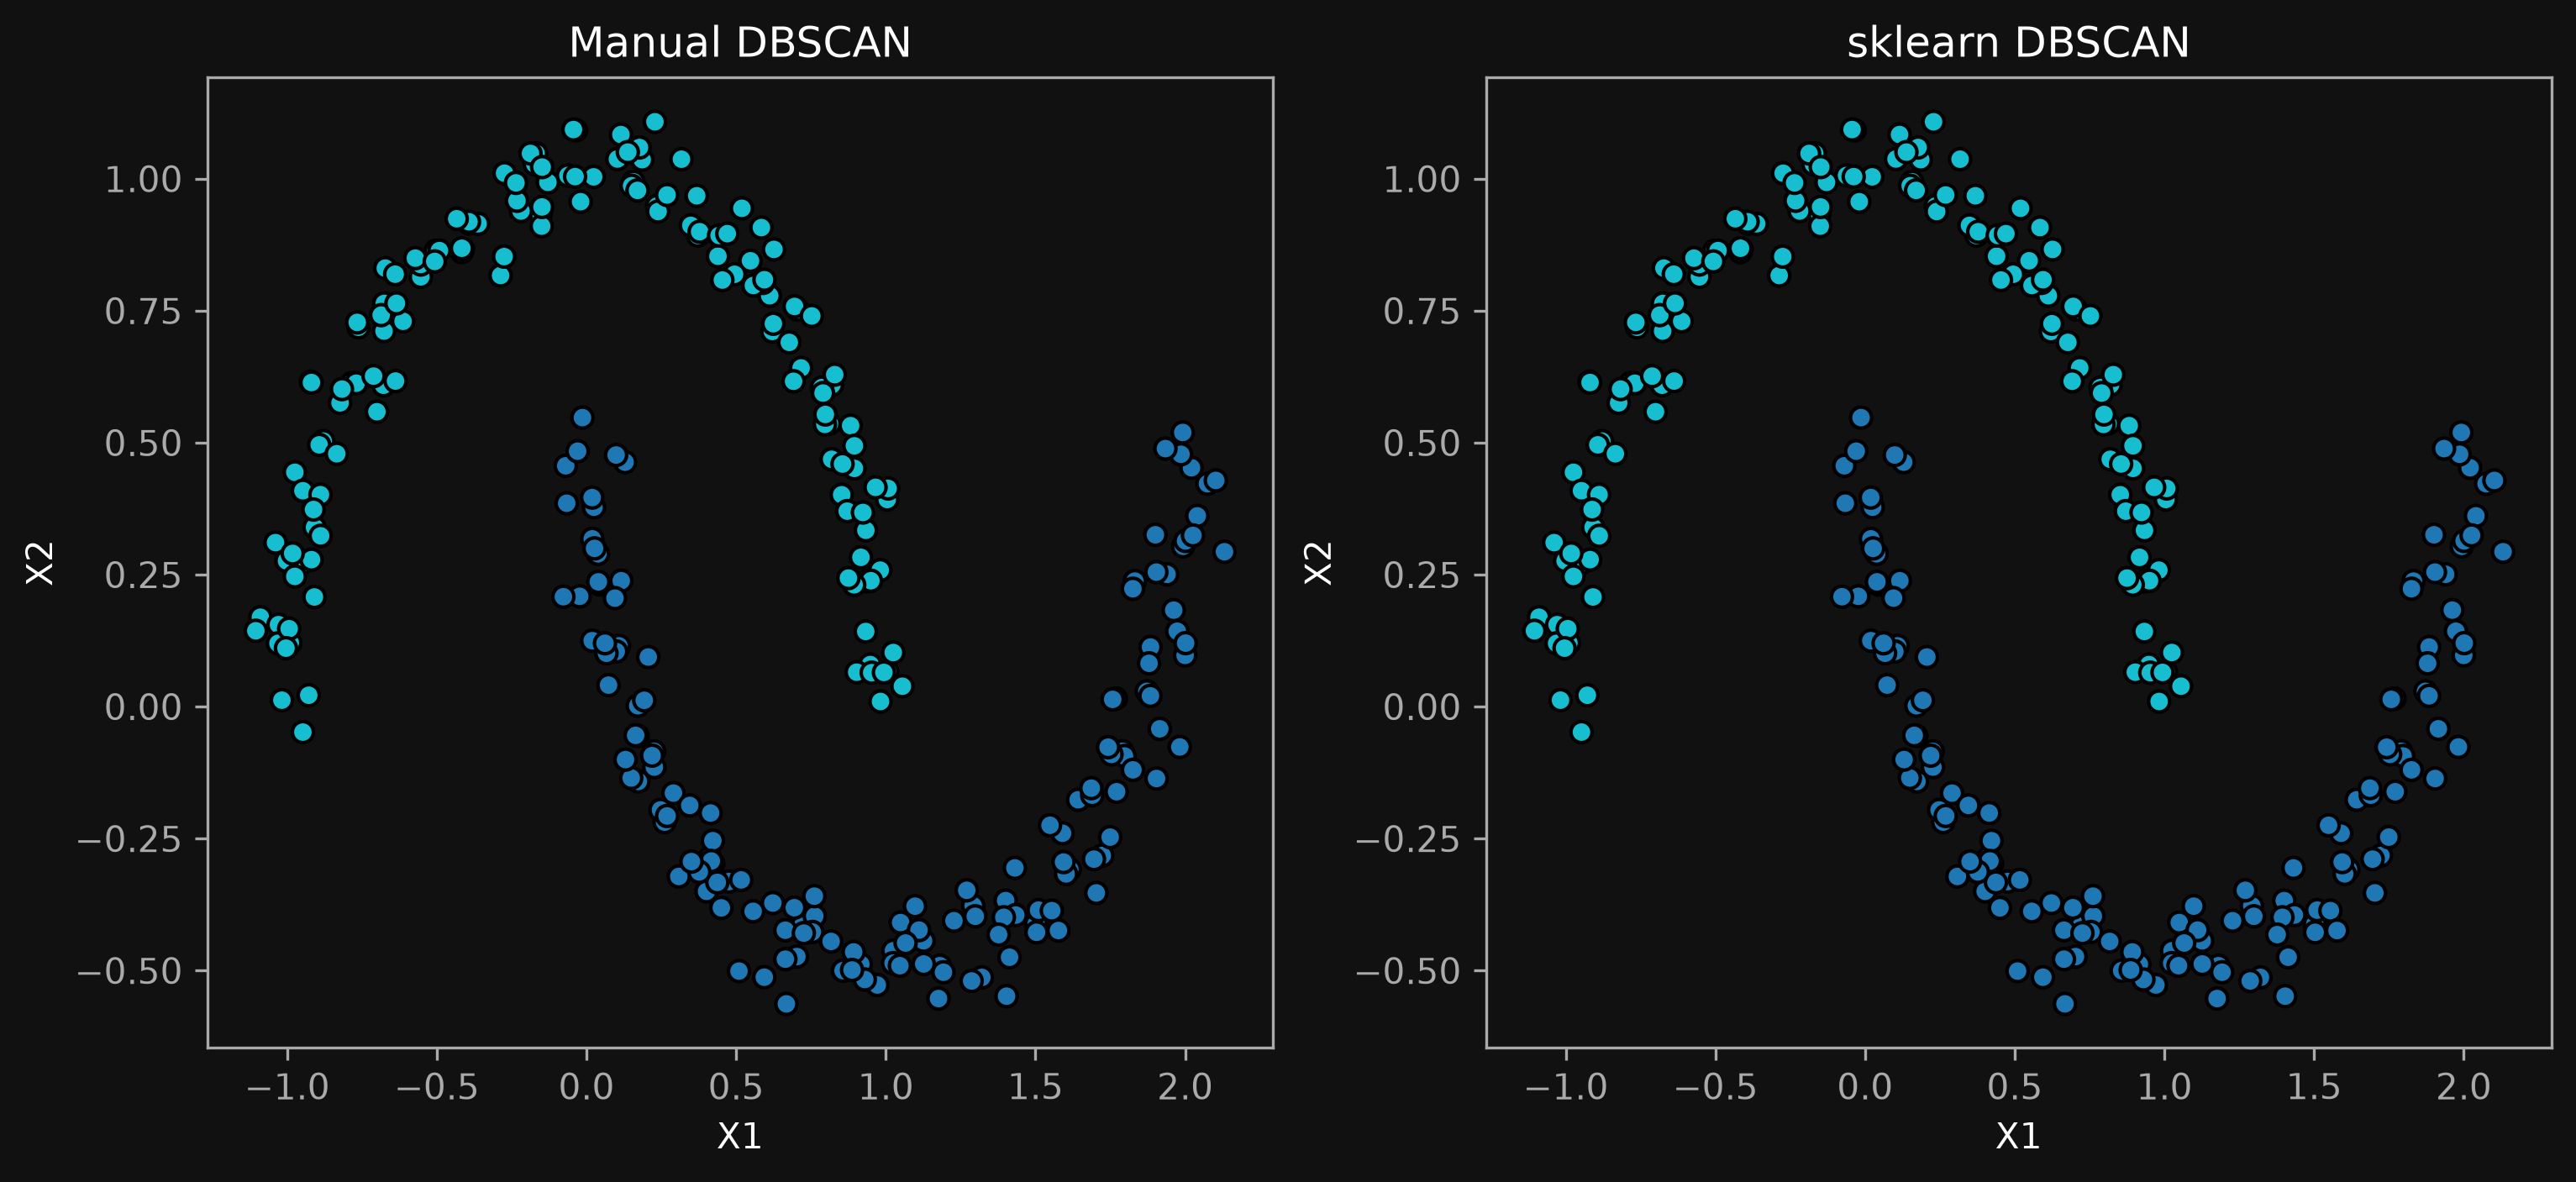
\includegraphics[width=0.95\textwidth]{./figures/problem6_dbscan_comparison.png}
\end{center}

DBSCAN separates the two moons, which K-means cannot: the moons interlock, so no pair of centroids
splits them. DBSCAN never assumes a shape, only that cluster members are reachable through a chain
of $\epsilon$-neighbors.


\end{document}